\chapter{Python dan Anaconda}
\section{Teori}
\subsection{Sejarah Python}
\hspace{0,5cm} Bahasa Pemrograman python ada pada tahun 1980 oleh Guido van Rossum di CWI Belanda. Van Rossum  adalah penulis utama Python, kemudian pada tahun 2000 python merilis versi 2.0 dangan memiliki banyak fitur yang baru, seperti cycle-detecting garbage collector untuk mengotomasi manajemen memori. Versi 2.0 dinilai lebih transparan dan inklusif untuk pengembangan software ketimbang versi sebelumnya. Hal ini didukung dengan adanya PEP – Python Enhancement Proposal, sebuah spesifikasi teknis yang menjadi tuntunan informasi untuk penggunanya dan menggambarkan fitur baru pada Python.\\
\par Python versi 3.0 adalah versi dengan banyak perubahan, termasuk memasukkan statemen print ke dalam built-in function. Python vesi 3.0 dirilis pada akhir tahun 2008. Python 2.7 dirilis pada tahun 2010 yang bertujuan agar pengguna python versi 2 mudah berpindah ke python versi 3.\\
\subsection{Iplementasi dan Penggunaan Python pada Perusahaan}
\par Iplementasi penggunaan python pada perusahaan adalah sebagai berikut :

\begin{enumerate}
\item Ketersediaan akan open-source library, frameworks, tools untuk data mining, contohnya adalah SciKit Learn, TensorFlow, Keras.
\item Relatif lebih mudah dipahami. Penulisan code di Python relatif lebih singkat.
\item Multifungsi, tidak hanya untuk data processing, namun juga bisa untuk tugas lain seperti membuat website dan tampilan GUI (Graphical User Interface).
\end{enumerate}


\section{Instalasi}

\begin{enumerate}
\item Instalasi Python 3
\begin{itemize} 
\item Download python sesuai dengan OS yang di pakai, anda dapat mengunduh di https://www.python.org/downloads/release/python-370.
\item Kemudian Klik 2x pada file instalasi python.
\item Pilih Install Now.
\item Tunggu hingga selesai Instalasinya.
\end{itemize}


\item Instalasi PIP

\begin{itemize} 
\item Download PIP sesuai dengan versi python yang di pakai, anda dapat mengunduh PIP di https://pypi.org/project/pip/files.
\item Kemudian klik 2 kali pada get-pip.py atau setup.
\item Kemudian masuk ke Control Panel - System And Security - System - Advanced System Settings
\item Lalu klik Environment Variables, pada sesi System Variables pilih path - Edit - New - C:/Python3/Scripts - Ok.
\item Buka Command Prompt, kemudian ketik PiP.
\item Selesai
\end{itemize}


\item Setting Environment

\begin{itemize} 
\item Masuk ke Control Panel - System And Security - System - Advanced System Settings
\item Lalu klik Environment Variables, pada sesi System Variables pilih path - Edit - New - C:/Python3/Scripts - Ok.
\end{itemize} 


\item Mencoba entrepriter/CLI pada terminal atau cmd

\begin{itemize}
\item Buka terninal atau cmd.
\item Ketik python pada cmd atau terminal.
\item Kemudian untuk print sebuah text anda tinggal menambahkan text print ("Hello world!").
\end{itemize}


\item Menjalangkan dan mengupdate Anaconda dan Spyder

\begin{itemize}
\item Dowonload anaconda di https://www.anaconda.com/distribution.
\item Install anaconda.
\item Jika sudah di install, selanjutnya lansung buka anacondanya dengan mengklik 2x.
\item Pada menu utama aplikasi anaconda maka akan terdapat beberapa tools yang disediakan, termasuk spyder dan lain-lain.
\end{itemize}


\item Cara Menjalangkan Script Hello Word di spyder
\begin{itemize}
\item Pertama anda membuka aplikasi spyder, kemudian tambahkan scrip seperti pada gambar berikut.
	\begin{figure}
		\begin{center}
			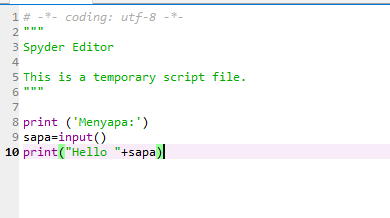
\includegraphics[width = 10cm, height= 7cm]{gambar_1.PNG}
			\caption{gambar 1}
		\end{center}
	\end{figure}
\end{itemize}



\end{enumerate}
\end{document}